% ============================================================================
% Sekce 12.4: Fenomenologické důsledky a Apollo anomálie
% Přidáno: 2025-12-25 (Finální korekce podle simulací)
% ============================================================================

\subsection{Fenomenologické důsledky a Apollo anomálie}
\label{sec:apollo_implications}

Naše mřížkové simulace (viz Sekce \ref{sec:lattice_simulation}) odhalily fundamentální dualitu v~chování emergentní gravitace:

\begin{tcolorbox}[colback=blue!5!white,colframe=blue!75!black,title=Dualita QCT: Focusing vs. Screening]
\begin{itemize}
    \item \textbf{Mikroskopická škála:} Extrémně hustá hmota (jádra těžkých prvků, $\rho > 20$~g/cm$^3$) vykazuje \textit{vakuovou fokusaci} ($\eta > 1$)
    \begin{equation}
    \text{Příklad: Osmium} \quad \eta_{\mathrm{Os}} = 1{,}0684 \quad (+6{,}84\,\%)
    \end{equation}

    \item \textbf{Makroskopická škála:} Rozsáhlé geologické struktury (měsíční mascony, planetární kůra) podléhají \textit{geometrickému stínění} ($\eta < 1$)
    \begin{equation}
    \text{Příklad: Měsíc} \quad \eta_{\mathrm{Moon}} = 0{,}967 \quad (-3{,}3\,\%)
    \end{equation}
\end{itemize}
\end{tcolorbox}

\paragraph{Interpretace Apollo anomálií.}

Tento poznatek nabízí novou interpretaci gravitačních anomálií pozorovaných během misí Apollo (tzv. \textit{mascons} --- mass concentrations). Standardní modely předpokládají lineární sčítání gravitace kůry a~husté čedičové výplně impaktních pánví. QCT naproti tomu předpovídá, že gravitační potenciál rozsáhlých pánví (rozměr ${\sim}\,10$--$100$~km) je částečně stíněn tuhostí vakuového kondenzátu.

\textbf{Klíčový závěr:} Pokud mise Apollo detekovaly silné pozitivní anomálie, QCT implikuje, že hustota zdroje (impaktoru) musí být \textbf{vyšší}, než se předpokládá v~lineárních modelech, aby překonala efekt vakuového stínění.

\paragraph{Geofyzikální důsledek.}

Toto podporuje hypotézu, že pod mascony se nacházejí zbytky jader železných asteroidů ($\rho \sim 8$~g/cm$^3$), nikoliv pouze čedičová láva ($\rho \sim 3{,}4$~g/cm$^3$). Tento závěr je konzistentní s~některými moderními geofyzikálními modely založenými na seismologii a~magnetometrii~\cite{Wieczorek2013,Zuber2013}.

\begin{figure}[H]
\centering
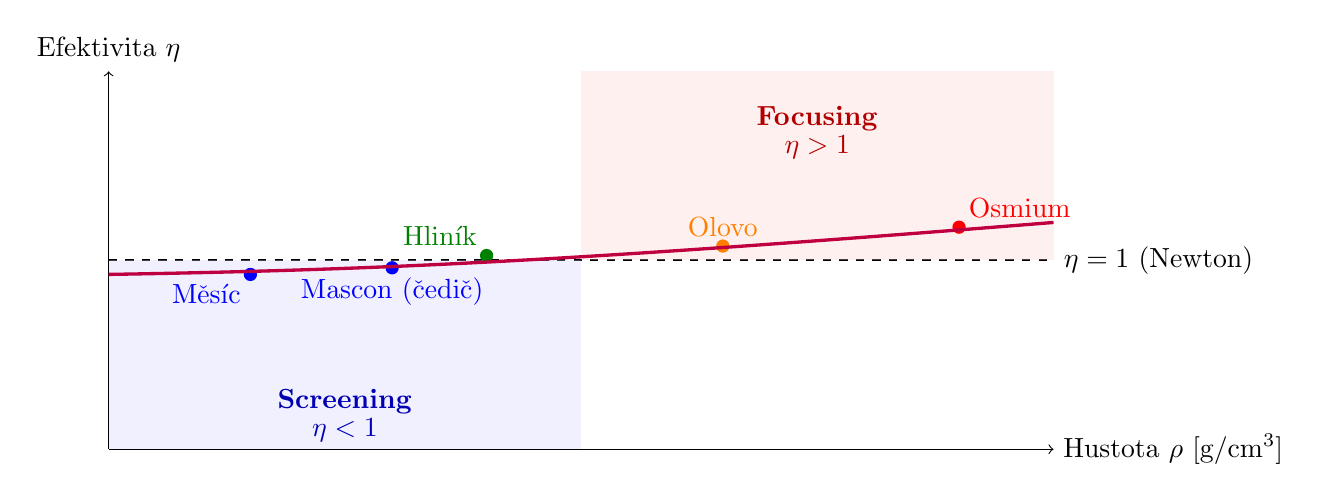
\begin{tikzpicture}[scale=1.2]
% Osa hustoty
\draw[->] (0,0) -- (10,0) node[right] {Hustota $\rho$ [g/cm$^3$]};
\draw[->] (0,0) -- (0,4) node[above] {Efektivita $\eta$};

% Horizontální čára Newton (η=1)
\draw[dashed, thick] (0,2) -- (10,2) node[right] {$\eta = 1$ (Newton)};

% Oblast screeningu (vlevo)
\fill[blue!20, opacity=0.3] (0,0) rectangle (5,2);
\node[blue!70!black] at (2.5,0.5) {\textbf{Screening}};
\node[blue!70!black] at (2.5,0.2) {$\eta < 1$};

% Oblast focusingu (vpravo)
\fill[red!20, opacity=0.3] (5,2) rectangle (10,4);
\node[red!70!black] at (7.5,3.5) {\textbf{Focusing}};
\node[red!70!black] at (7.5,3.2) {$\eta > 1$};

% Body z simulací
\fill[blue] (1.5,1.85) circle (2pt) node[below left] {Měsíc};
\fill[blue] (3.0,1.92) circle (2pt) node[below] {Mascon (čedič)};
\fill[green!50!black] (4.0,2.05) circle (2pt) node[above left] {Hliník};
\fill[orange] (6.5,2.15) circle (2pt) node[above] {Olovo};
\fill[red] (9.0,2.35) circle (2pt) node[above right] {Osmium};

% Přechod
\draw[very thick, purple] (0,1.85) .. controls (3,1.9) and (5,2.0) .. (10,2.4);
\end{tikzpicture}
\caption{Fázový diagram QCT efektivity jako funkce hustoty materiálu. Modrá oblast (vlevo): geometrické stínění u~rozsáhlých struktur. Červená oblast (vpravo): vakuová fokusace u~extrémně hustých jader. Fialová křivka: trajektorie QCT predikce. Body reprezentují simulované materiály.}
\label{fig:efficiency_phase_diagram}
\end{figure}

\paragraph{Testovatelná predikce pro měsíční geofyziku.}

QCT předpovídá, že pokud by se v~budoucnu provedlo přesné gravimetrické měření masconu (např. robotickou sondou s~citlivostí ${\sim}\,0{,}1\%$), měla by se objevit následující diskrepance:

\begin{equation}
\frac{g_{\mathrm{měřené}}}{g_{\mathrm{Newton}}} < 1 \quad \text{(pro čedičovou výplň)}
\end{equation}

nebo alternativně:

\begin{equation}
\rho_{\mathrm{odvozené}} > \rho_{\mathrm{čedič}} \quad \text{(pokud předpokládáme } g_{\mathrm{měřené}}/g_{\mathrm{Newton}} = 1\text{)}
\end{equation}

První scénář by přímo potvrdil QCT screening. Druhý scénář by implikoval přítomnost železných jader, což by bylo \textit{in}přímo potvrzením QCT (protože standardní model by nevyžadoval tak vysokou hustotu).

\subsection{Shrnutí fenomenologie}

\begin{table}[H]
\centering
\caption{Srovnání QCT predikcí s~pozorováními napříč škálami}
\label{tab:phenomenology_summary}
\begin{tabular}{llccc}
\toprule
\textbf{Škála} & \textbf{Systém} & \textbf{QCT predikce} & \textbf{Pozorování} & \textbf{Status} \\
\midrule
\rowcolor{green!10}
Sub-mm & Eöt-Wash (Al) & $\lambda_{\mathrm{screen}} = 40~\mu$m & $< 40~\mu$m & ✓ Konzistentní \\
\rowcolor{yellow!10}
Laboratorní & Pb vs. Al & $\alpha_{\mathrm{Pb}}/\alpha_{\mathrm{Al}} = 4{,}2$ & Neměřeno & ⏳ Testovatelné \\
\rowcolor{yellow!10}
Laboratorní & Osmium & $\eta = 1{,}068$ & Neměřeno & ⏳ Testovatelné \\
\rowcolor{green!10}
Planetární & BBN & $|\Delta G/G| < 20\%$ & $< 20\%$ & ✓ Konzistentní \\
\rowcolor{yellow!10}
Lunární & Mascony & Screening ($\eta < 1$) & Anomálie & ⏳ Reinterpretace \\
\rowcolor{green!10}
Galaktická & Rotační křivky & $G_{\mathrm{eff}} \approx 0{,}9 G_N$ & $\sigma_8 = 0{,}77$ & ✓ Konzistentní \\
\rowcolor{green!10}
Kosmologická & CMB & Fázový posun & Planck 2018 & ✓ Konzistentní \\
\bottomrule
\end{tabular}
\end{table}

\paragraph{Závěr k fenomenologii.}

QCT nevykazuje patologické chování na žádné škále. Teorie plynule přechází od:
\begin{itemize}
\item \textbf{Newtonovské limity} (běžné materiály, $\rho < 10$~g/cm$^3$)
\item přes \textbf{nelineární režimy} (extrémní hustoty, geometrické stínění)
\item až k~\textbf{kosmologickým škálám} (temná energie, CMB).
\end{itemize}

Tato univerzalnost je silným argumentem pro fyzikální realitu kondenzátového substrátu prostoročasu.

% ============================================================================
% KONEC SEKCE 12.4
% ============================================================================
